\pstart 
[99 v\textsuperscript{o}] \textso{Gerick. lib. }[\textso{4}]\edtext{}{\lemma{\textso{3}}\Afootnote{\textit{\ L \"{a}ndert Hrsg. } }}\textso{ c. 4 }\edtext{}{\lemma{4}\Bfootnote{\textsc{O. v. Guericke, }\cite{00055}a.a.O., S.~131f.}} Kircherus\protect\index{Namensregister}{\textso{Kircher} (Kircherus), Athanasius SJ 1602\textendash 1680} lib 2. \textit{magnet}.  1. progymn. prop. 5. pragm. 3. pag. 157\edtext{}{\lemma{157}\Bfootnote{\textsc{A. Kircher, }\cite{00067}\textit{Magnes}, Rom 1654, S.~118.}}  modum invenit sphaerulam exacte librandi  in media sphaera vitrea aqua fontana vel  alio liquore longa decoctione a faece turbida  separato, unde heterogeneo immiscibili sed  concolori ut \textit{e vino, therebinto baccis been vel simili} superfuso. Ego inquit Kircherus\protect\index{Namensregister}{\textso{Kircher} (Kircherus), Athanasius SJ 1602\textendash 1680} \textit{spiritum tartari spiritui vini cui misceri nequit  conjungere soleo. }\textit{Magnetem}\protect\index{Sachverzeichnis}{magnes}\textit{ autem fundo vel  orificio vasis ita aptat ut }\textit{poli}\protect\index{Sachverzeichnis}{polus}\textit{ ejus horizonti  aequidistent, ita sphaerula ex }\textit{magnete}\protect\index{Sachverzeichnis}{magnes}\textit{  facta a }\textit{magnete}\protect\index{Sachverzeichnis}{magnes}\textit{ jam memorato semper  in medium vasis centrum trahitur, ut se }\textit{poli}\protect\index{Sachverzeichnis}{polus}
\textit{ conforment.} 
At Gerickius\protect\index{Namensregister}{\textso{Guericke} (Gerickius, Gerick.), Otto v. 1602\textendash 1686} alium  invenit modum suo scopo aptiorem, ut ostenderet Telluris\protect\index{Sachverzeichnis}{tellus} lationem annuam circa Lunam\protect\index{Sachverzeichnis}{luna}.\edtext{}{\lemma{Lunam.}\Bfootnote{Bei Guericke: Solem\protect\index{Sachverzeichnis}{sol}}}  Primum \textso{aqua a putredine praeservanda,} quod  fit si dolium seu vas aqua refertum pluvia, soli\protect\index{Sachverzeichnis}{sol} exponatur per totam aestatem ut putrescat  una vel altera vel tertia vice, ita ut in eo  vermiculi multi et varii generentur deinde hyeme in cella a gelu tuta conservata, secunda aestate  iterum soli\protect\index{Sachverzeichnis}{sol} exponitur, tandemque per papyrum  in vitreum aliquod vas quod pharmacopolae $\displaystyle \frac{1}{4}\rule[-4mm]{0mm}{10mm}$% \begin{wrapfigure}{l}{0.4\textwidth}                    
                %\includegraphics[width=0.4\textwidth]{../images/Aus+Otto+von+Guericke%2C+Experimenta+nova/LH035%2C14%2C02_099v/files/100185.png}
                        %\caption{Bildbeschreibung}
                        %\end{wrapfigure}
                        %@ @ @ Dies ist eine Abstandszeile - fuer den Fall, dass mehrere figures hintereinander kommen, ohne dass dazwischen laengerer Text steht. Dies kann zu einer Fahlermeldung fuehren. @ @ @ \\
                      \ recipientem vocant infunditur. Debet vitreum  hoc vas inferiori parte cum agglutinata lamina  ut et cuspide ferrea ita esse instructum, ut  super cuspidem tanquam axem mediantibus  (a superiore parte) aliquibus rotis horologiariis quasi possit lente rotari. Postea sphaeram  aeneam vel vitream magnitudine dimidii ovi  accommoda in aequali pondere cum aqua; quod  fieri potest, quando in sphaerulam aliquod aquae  calidae infunditur, et deinde sphaera\edtext{}{\lemma{sphaera}\Bfootnote{Bei Guericke: cera}} bene  clauditur, tandem haec cera aliquibus plumbi  frustulis oneratur, ita ut sphaerula ipsi aquae gravitati\protect\index{Sachverzeichnis}{gravitas} sit adaequata nec ullam  in aqua habeat gravitatem\protect\index{Sachverzeichnis}{gravitas} vel levitatem\protect\index{Sachverzeichnis}{levitas}  sed libere pendeat. Sed certa temperiei  constitutio est observanda, nam quando calido  tempore id perficis, sphaera facile fundum  petit, tempore frigidiori innatabit unde quando  innatat et in locum calidiorem fertur, sphaerula  lente descendit ad medium, aut secundum aquae  temperamentum iterum ascendet, vel denique fundum  petet, quando vero fundum petit, debet vitrum  in frigidiorem locum reportari, tunc ascendet  sphaerula. Quando jam in ascensu aut descensu, vel quod melius in lenta\edtext{}{\lemma{lenta}\Bfootnote{Bei Guericke: quieta}} statione est,  tunc potest vas lente in gyrum moveri, et sphaerula tandem se fert ad ampliorem locum id  est mediam circumferentiam, et quanquam  propter acceptum impulsum vel supra vel infra aequatorem\protect\index{Sachverzeichnis}{aequator} ad quasi Tropicos\protect\index{Sachverzeichnis}{tropicus} declinet,\edtext{}{\lemma{declinet,}\Bfootnote{Bei Guericke: inclinet}} tamen cogitur redire propter angustiorem locum quia versus axem vel polos\protect\index{Sachverzeichnis}{polus} virtus arctaretur.  Excedunt enim omnia impulsa. Nec aliud vibrationes quam excessus.\pend\clearpage \pstart \textso{Gerick. lib. }[\textso{4.}]\edtext{}{\Afootnote{\textso{ 2.}\textit{\ L \"{a}ndert Hrsg. } }}\textso{ c. 7 }\edtext{}{\lemma{7}\Bfootnote{\textsc{O. v. Guericke}, \cite{00055}a.a.O., S.~135.}} virtus \textso{magnetica} per attritionem excitari potest in quovis ferro\protect\index{Sachverzeichnis}{ferrum}. \textit{Accipe  filum ferreum longitudine digiti, et concute ejus  terminos malleo super incude secundum lineam  meridianam, ita ut unus fili terminus septentrionem  alius austrum versus dirigatur, et videbis illud  se disponere ut }\textit{acum}\protect\index{Sachverzeichnis}{acus!magnetica}
                      \protect\index{Sachverzeichnis}{acus|see{aiguille aimant\'{e}e}}
                      \textit{ seu }\textit{lingulam magneticam}\protect\index{Sachverzeichnis}{lingula magnetica}\textit{.  Unde armamentula ista Chalybea, quibus fabri perforant }\textit{ferrum}\protect\index{Sachverzeichnis}{ferrum}\textit{ et vulgo hordei grana  Germanice Gersten Korner vocantur ob  durum istum attritum saepius iteratum  hanc quoque virtutem acquirunt, et limaturas  ferreas copiose attrahunt. Recipe  ex }\textit{horologio}\protect\index{Sachverzeichnis}{horologium}\textit{ aliquo solari acum vel lingulam }\textit{magneticam}\protect\index{Sachverzeichnis}{lingula magnetica}\textit{, impone super aciculam ut libere  possit vagari et applica ad }\textit{\textso{Lapidem}} cujus polos\protect\index{Sachverzeichnis}{polus} quaeris, tunc pars septentrionalis acus  ostendet polum australem\protect\index{Sachverzeichnis}{polus!australis} lapidis et contra  postea per cotem exacuatur juxta suos polos  in formam ovalem, et aptus erit imbuendis  aliis acus\protect\index{Sachverzeichnis}{acus}.\pend \pstart  cap. 9.\edtext{}{\lemma{9.}\Bfootnote{\textsc{O. v. Guericke}, \cite{00055}a.a.O., S.~137.}}\edtext{}{\lemma{9.}\Bfootnote{In den \textit{Experimenta nova}  irrt\"{u}mlich als Cap. 13 ausgewiesen.}} virtute vertente Telluris\protect\index{Sachverzeichnis}{tellus}  circumagitur et Luna\protect\index{Sachverzeichnis}{luna}, et quia remotior, non  eodem tempore sed quod terra\protect\index{Sachverzeichnis}{terra} in 24 horis, Lunam\protect\index{Sachverzeichnis}{luna} $\displaystyle 29\frac{1}{2}\rule[-4mm]{0mm}{10mm}\hspace{5.5pt}$% \begin{wrapfigure}{l}{0.4\textwidth}                    
                %\includegraphics[width=0.4\textwidth]{../images/Aus+Otto+von+Guericke%2C+Experimenta+nova/LH035%2C14%2C02_099v/files/100442.png}
                        %\caption{Bildbeschreibung}
                        %\end{wrapfigure}
                        %@ @ @ Dies ist eine Abstandszeile - fuer den Fall, dass mehrere figures hintereinander kommen, ohne dass dazwischen laengerer Text steht. Dies kann zu einer Fahlermeldung fuehren. @ @ @ \\
                     diebus (+ hoc conferatur cum  distantia terrae\protect\index{Sachverzeichnis}{terra} a sole\protect\index{Sachverzeichnis}{sol}, et consideretur an  sit et jam possit \edtext{solaris vertiginis}{\lemma{possit}\Afootnote{ \textit{ (1) }\ rotationis \textit{ (2) }\ solaris vertiginis \textit{ L}}}  periodus +).
                     \pend
                      \pstart 
                      \textso{c. 10.}\edtext{}{\lemma{\textso{10.}}\Bfootnote{\textsc{O. v. Guericke}, \cite{00055}a.a.O., S.~139f.}} Urinatores profunde intra  aquam demissi audiunt sonos\protect\index{Sachverzeichnis}{sonus} vehementes. Echo  putat non a \edtext{figura loci, sed}{\lemma{a}\Afootnote{ \textit{ (1) }\ virtute, sed \textit{ (2) }\ figura loci, sed \textit{ L}}} qualitate\edtext{}{\lemma{qualitate}\Afootnote{ \textbar\ soni \textit{ gestr.}\ \textbar\ pendere, \textit{ L}\protect\rule[0cm]{2cm}{0cm}}} pendere, uti lapis bononiensis\protect\index{Sachverzeichnis}{lapis!bononiensis} lucem\protect\index{Sachverzeichnis}{lux} bibit,  et reddit, ita Echo, ait, sonum\protect\index{Sachverzeichnis}{sonus}, certum petrae  genus forte ad id aptum esse. Hanc materiam forte esse  ut os petrosum in animalium\protect\index{Sachverzeichnis}{animal} auribus.
                      \pend 
                      \pstart \textso{c. 11.}\edtext{}{\lemma{\textso{11.}}\Bfootnote{\textsc{O. v. Guericke}, \cite{00055}a.a.O., S.~141.}} Circa  Lacrymas vitri gl\"{a}serne Springkhornlein\protect\index{Sachverzeichnis}{Springkhornlein}, quas nunquam sibi visas  ait ejusdem mecum sententia est.\pend \pstart \textso{c. 12.}\edtext{}{\lemma{\textso{12.}}\Bfootnote{\textsc{O. v. Guericke}, \cite{00055}a.a.O., S.~142.\protect\rule[0cm]{6cm}{0cm}}} \textit{Caeruleus }\textit{color}\protect\index{Sachverzeichnis}{color}\textit{ in superiore  aeris parte oritur ex nigro et albo; ubi enim aer  a rarissimis aquosis humoribus desinit vel omnino purus  fit, ibi deficit album ut incipit nigrum.} Nam  purus aer lumen\protect\index{Sachverzeichnis}{lumen} liberrime transmittit seu niger  est. Hinc gutta lactis et atramenti ad invicem  posito in loco intermedio (+ \textso{NB} ita alii colores sibi  sine commixtione tantum admoveri possunt,  ut appareat quis color\protect\index{Sachverzeichnis}{color} ex eorum umbris, ita lux\protect\index{Sachverzeichnis}{lux} per diversa colorata in eundem locum trajici  et ita colores\protect\index{Sachverzeichnis}{color} misceri +) caeruleum efficiunt colorem\protect\index{Sachverzeichnis}{color}  (+ an forte et caeteri ex nigro et albo, nam ex flavo  et caeruleo viridis +).
                      \pend                 
                       \begin{center}        
                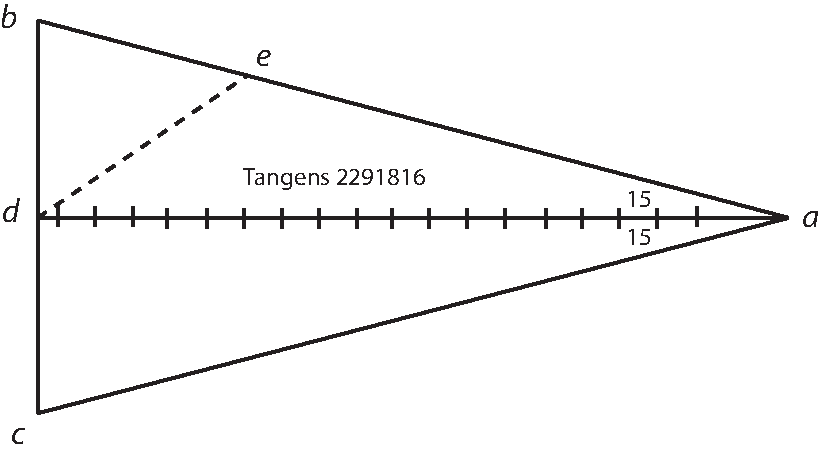
\includegraphics[width=0.8\textwidth]{images/99v}\\\textit{[Fig. 2]}
                        %\caption{Bildbeschreibung}
                        \end{center}
                        \pstart 
       \textso{cap. 13.} \edtext{}{\lemma{\textso{13.}}\Bfootnote{\textsc{O. v. Guericke}, \cite{00055}a.a.O., S.~142\textendash144.}} \textit{De natura et qualitatibus visus.} Ibi Gerickius\protect\index{Namensregister}{\textso{Guericke} (Gerickius, Gerick.), Otto v. 1602\textendash 1686} de distantia ex
                                  diametro apparente cognoscenda. Sed distantiae  ratio haberi potest non \edtext{absoluta  sed ad ipsius}{\lemma{non}\Afootnote{ \textit{ (1) }\ ad ipsam \textit{ (2) }\ absoluta  sed ad ipsius \textit{ L}}} astri magnitudinem. Nam esto 
                        %@ @ @ Dies ist eine Abstandszeile - fuer den Fall, dass mehrere figures hintereinander kommen, ohne dass dazwischen laengerer Text steht. Dies kann zu einer Fahlermeldung fuehren. @ @ @ \\
                      angulus \textit{bac} \edtext{30. min.}{\lemma{30.}\Afootnote{ \textit{ (1) }\ grad. \textit{ (2) }\ min. \textit{ L}}} erit \textit{dab} \edtext{15. min.}{\lemma{15.}\Afootnote{ \textit{ (1) }\ grad. \textit{ (2) }\ min. \textit{ L}}} centro \textit{b} radio \textit{bd} describatur arcus \textit{de} hujus tangens \textit{da}  quae est 229. si \textit{bd}  est 1. seu erit 2291816  si \textit{bd} est 1,0000.\edtext{}{\lemma{}\Afootnote{1,0000.  \textbar\ Notam \textit{da} esse \textit{streicht Hrsg.}\ \textbar\ Ergo \textit{ L}}}  Ergo si objecti magnitudo nobis cognita  omnia determinari possunt. 
                      \pend